%% PLEM paper -- structural skeleton.
%% Every section, subsection, label, table and figure of main.tex, with no body text.
%% What each part must say is in section_points.md (same directory).
%% Compiles on its own (set it as the main document in Overleaf, or compile it directly);
%% \nocite{*} keeps the reference list so BibTeX has citations to process.

\documentclass[sigconf]{acmart}

\usepackage{booktabs}
\usepackage{amsmath}
\usepackage{graphicx}
\usepackage{array}

\bibliographystyle{ACM-Reference-Format}
\citestyle{acmauthoryear}

\setcopyright{acmlicensed}
\copyrightyear{2026}
\acmYear{2026}
\acmDOI{10.1145/XXXXXXX.XXXXXXX}
\acmConference[SIGSPATIAL '26]{The 34th ACM SIGSPATIAL International Conference on Advances in Geographic Information Systems}{November 3--6, 2026}{Riverside, CA, USA}
\acmBooktitle{The 34th ACM SIGSPATIAL International Conference on Advances in Geographic Information Systems (SIGSPATIAL '26), November 3--6, 2026, Riverside, CA, USA}
\acmISBN{978-1-4503-XXXX-X/26/11}

%% Placeholder marker for body text still to be written.
\newcommand{\tbd}[1]{\textcolor{gray}{[#1]}}

\begin{document}

\title{PLEM: Polygonal Linear Evaluation Metric}
\subtitle{Evaluation Metrics and a Differentiable Training Loss for Joint Point, Linear, and Polygonal Map Feature Extraction}

\author{Daniel George}
\email{dzgeorge@usc.edu}
\affiliation{%
  \institution{University of Southern California, Viterbi School of Engineering}
  \city{Los Angeles}
  \state{CA}
  \country{USA}
}

\author{John Krumm}
\email{jkrumm@usc.edu}
\affiliation{%
  \institution{University of Southern California, Viterbi School of Engineering}
  \city{Los Angeles}
  \state{CA}
  \country{USA}
}

\begin{abstract}
\tbd{Problem: IoU fails on linear features. Metrics: DTAF1, CBHM, cbhm\_soft, DTAF1-Topo.
Loss: PLEMMultiTaskLoss and masked multi-source training. Results: production run, matched
baseline. Lessons from the six development runs.}
\end{abstract}

\keywords{geospatial segmentation evaluation, road extraction, building extraction,
tolerance-radius metrics, topology-aware metrics, centerline Dice, boundary F1, Average Path
Length Similarity, multiclass segmentation, differentiable loss functions, multi-task learning,
point/keypoint detection, soft-skeletonization}

\maketitle

%% ===================================================================== 1
\section{Introduction}
\label{sec:intro}

\tbd{Three feature types; point = road intersection.}

\tbd{IoU and CE/Dice are geometry-agnostic.}

\begin{table*}
  \caption{IoU and DTAF1 failure modes for linear and polygonal features.}
  \label{tab:failure-modes}
  %% Columns: Scenario | Road IoU | clDice | DTAF1 | CBHM | CBHM-soft | Correct read
  %% Rows: perfect, road shifted 5px, road 3.3x thick, 33% road deleted,
  %%       building eroded 5px, sparse road offset, null
\end{table*}

\tbd{Data representation and GSD-tied tolerances.}

\tbd{Contributions (numbered list).}

\tbd{Paper organization.}

%% ===================================================================== 2
\section{Related Work}
\label{sec:related}

\subsection{IoU-family segmentation metrics}
\tbd{}

\subsection{Topology-/skeleton-aware metrics for linear structures}
\tbd{}

\subsection{Boundary-based metrics for polygonal features}
\tbd{}

\subsection{Road-network extraction and connectivity metrics}
\label{subsec:related-roads}
\tbd{}

\subsection{Point/instance detection metrics}
\tbd{}

\subsection{Composite/multi-task segmentation evaluation}
\tbd{}

\subsection{Differentiable segmentation losses}
\label{subsec:related-losses}
\tbd{}

%% ===================================================================== 3
\section{Evaluation Protocol}
\label{sec:evalprotocol}

\tbd{Overview, shared notation, shared empty-mask convention.}

\subsection{DTAF1 --- Distance-Tolerant, per-class F1}
\label{subsec:dtaf1}
%% Eqs: TP_pred, TP_gt, precision/recall, F1_c; macro and weighted reductions.
\tbd{}

\subsection{clDice --- Centerline Dice}
\label{subsec:cldice}
%% Eqs: skeletons, T_prec, T_sens, clDice.
\tbd{}

\subsection{Boundary F1 (BF) and the IoU Baseline}
\label{subsec:bf}
%% Eqs: boundary precision/recall within tau, BF.
\tbd{}

\subsection{Point F1 --- Hungarian Instance Matching}
\label{subsec:pointf1}
\tbd{}

\subsection{APLS --- Raster-Skeleton Average Path Length Similarity}
\label{subsec:apls}
%% Eq: per-pair score max(0, 1 - |L_pred - L_gt| / L_gt).
\tbd{}

\subsection{CBHM --- Composite clDice/Boundary-F1 Harmonic Mean}
\label{subsec:cbhm}
%% Eqs: clDice_mean, BF_mean, CBHM.
\tbd{}

%% ===================================================================== 4
\section{Why These Metrics? Empirical Motivation}
\label{sec:motivation}

\subsection{Experimental Setup}
\label{subsec:motivation-setup}
\tbd{}

\begin{table}
  \caption{Synthetic sensitivity sweeps.}
  \label{tab:sweeps}
  %% Columns: Sweep | Perturbs | Range  (nine sweeps)
\end{table}

\subsection{Results}
\label{subsec:motivation-results}
\tbd{}

\subsection{Interpretation via Distance-Transform Geometry}
\label{subsec:motivation-interpretation}
\tbd{}

%% ===================================================================== 5
\section{Analysis and Design for Composite Robustness}
\label{sec:composite}

\subsection{Class-Imbalance--Controlled Tasks}
\label{subsec:class-imbalance}
\tbd{}

\subsection{Weighted Reduction as an Efficient Corrective Proxy}
\label{subsec:weighted-reduction}
%% Eq: cbhm_soft = w_linear * clDice_mean,weighted + w_polygon * BF_mean,weighted.
\tbd{}

\subsection{Choosing Per-Class Tolerance Radii}
\label{subsec:tolerance-radii}
\tbd{}

%% ===================================================================== 6
\section{Analysis and Design for Topological Robustness}
\label{sec:topological}

\subsection{The Connectivity Blind Spot}
\label{subsec:blindspot}
%% Formal statement (quote environment); proof in Appendix A.
\tbd{}

\subsection{APLS as Connectivity Recovery, and Its Sensitivity to Fragmentation}
\label{subsec:apls-recovery}
\tbd{}

\begin{table}
  \caption{Road-breakage sweep: DTAF1 vs.\ CBHM vs.\ APLS vs.\ DTAF1-Topo.}
  \label{tab:breakage-topo}
  %% Columns: Dropout | dtaf1 | cbhm | road_apls | dtaf1_topo  (fractions 0.0 ... 1.0)
\end{table}

\subsection{Harmonic-Blending Design for DTAF1-Topo}
\label{subsec:dtaf1topo}

\subsubsection{Closed-Form Boundary Behavior}
\tbd{}

\subsubsection{Numerical Validation via the Road-Breakage Sweep}
\tbd{}

\tbd{Bridge to Section~\ref{sec:method}.}

%% ===================================================================== 7
\section{A Differentiable Multi-Task Loss for Joint 0D/1D/2D Extraction}
\label{sec:method}

\tbd{Why the eval metrics cannot be losses; what losses/ is.}

\subsection{Design Principle: Differentiable Analogs, Not Shared Code}
\label{subsec:method-principle}
\tbd{}

\begin{table*}
  \caption{Eval metric $\leftrightarrow$ differentiable loss term correspondence.}
  \label{tab:correspondence}
  %% Columns: Eval metric | losses/ term | What changed to make it differentiable
  %% Rows: DTAF1, Boundary F1, clDice, Point F1, APLS/DTAF1-Topo (none)
\end{table*}

\subsection{Soft Tolerance-Band Loss (DTAF1 Analog)}
\label{subsec:tolerance-loss}
%% Eqs: gt_band, soft precision, soft recall, weighted loss.
\tbd{}

\subsection{Soft Boundary Loss (Boundary F1 Analog)}
\label{subsec:boundary-loss}
\tbd{}

\subsection{Soft-clDice Loss (clDice Analog)}
\label{subsec:cldice-loss}
%% Eqs: tprec, tsens, soft_clDice, loss.
\tbd{}

\subsection{Point-Heatmap Regression Loss (Point F1 Analog, Reformulated)}
\label{subsec:heatmap-loss}
%% Eqs: Gaussian target H, l+, l-, loss with N_pos and Z_neg.
\tbd{}

\subsection{PLEMMultiTaskLoss: Combination and Multi-Source Class Masking}
\label{subsec:multitask-loss}
%% Eqs: weighted sum L; logit masking.
\tbd{}

%% ===================================================================== 8
\section{Implementation}
\label{sec:implementation}

\tbd{Interfaces and return conventions.}

\begin{table}
  \caption{Tech stack, grouped by role.}
  \label{tab:techstack}
  %% Columns: Role | Libraries
\end{table}

%% ===================================================================== 9
\section{Experimental Setup}
\label{sec:expsetup}

\subsection{Synthetic Benchmark}
\label{subsec:synthetic-setup}
\tbd{}

\subsection{Real-Data Sample}
\label{subsec:realdata-setup}
\tbd{}

\subsection{Loss Ablation Setup}
\label{subsec:lossablation-setup}
\tbd{}

\subsection{Production Training Setup}
\label{subsec:scaled-setup}
\tbd{Model; development path; sources; road-intersection labels; building labels and coverage mask; training and
evaluation.}

\subsection{Conventional-Training Baseline Setup}
\label{subsec:baseline-setup}
\tbd{Loss; selection; intersection decoding; scoring; the two claims tested.}

%% ===================================================================== 10
\section{Results}
\label{sec:results}

\subsection{Synthetic Sensitivity Results}
\label{subsec:synthetic-results}
\tbd{}

\subsection{Real-Data Case Studies}
\label{subsec:realdata-results}
\tbd{}

\subsection{Loss Ablation Results}
\label{subsec:lossablation-results}
\tbd{}

\subsection{Production Training Results}
\label{subsec:scaled-results}

\begin{figure*}
  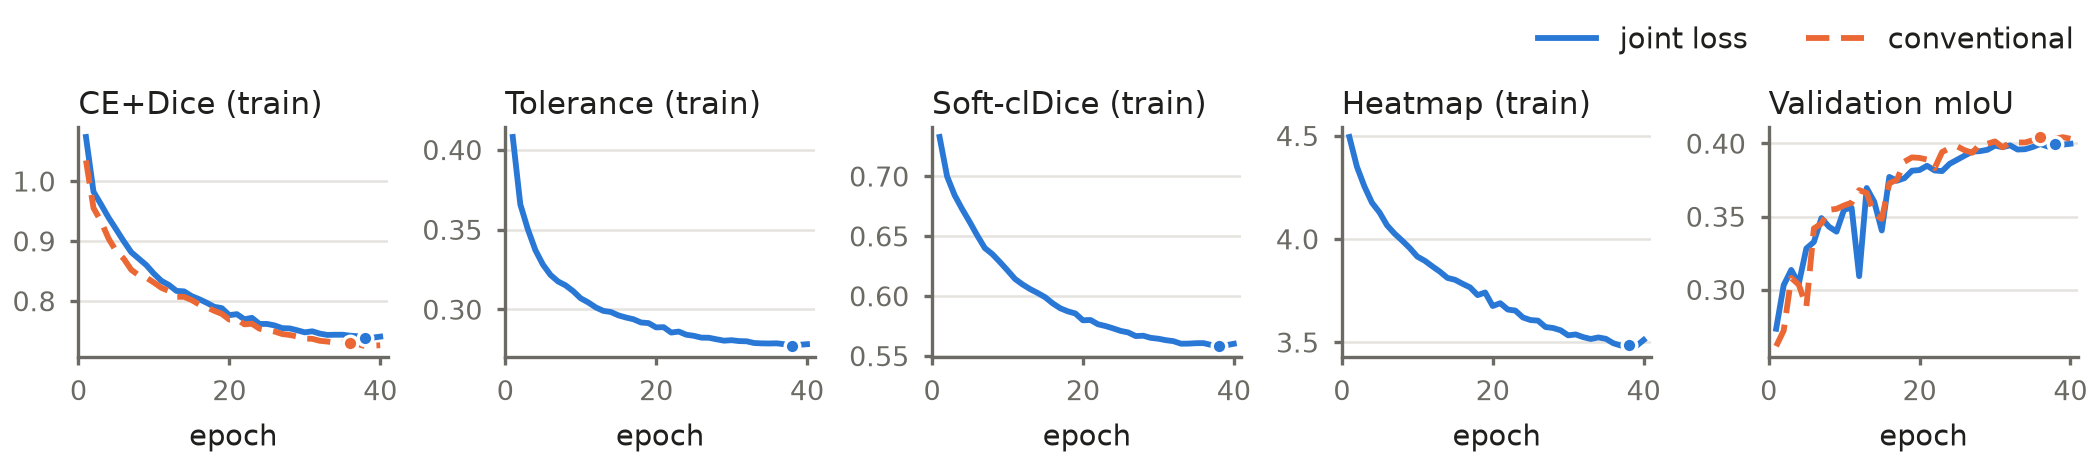
\includegraphics[width=\textwidth]{figures/training_curves.png}
  \Description{Training curves of the joint and conventional models over 40 epochs.}
  \caption{Training curves, joint loss vs.\ conventional baseline.}
  \label{fig:training-curves}
\end{figure*}

\begin{table*}
  \caption{Production model, test-set means per source.}
  \label{tab:scaled-test}
  %% Columns: Source (tiles) | cbhm_soft | cbhm | dtaf1_topo | dtaf1 | bf | cldice
\end{table*}

\tbd{Road intersections; separability; recall ceiling.}

\begin{table}
  \caption{Train/predict asymmetry: predicted pixels per class on the test tiles.}
  \label{tab:scaled-asymmetry}
  %% Columns: Source | Road px | Building px | Intersection px (inst.)
\end{table}

\tbd{Darkness. Development record.}

\begin{table*}
  \caption{Development record of the production pipeline.}
  \label{tab:scaled-history}
  %% Columns: Run | Point feature / head | cbhm (Potsdam / SpaceNet / SN6) | Point outcome |
  %%          Root cause -> fix   (runs 1-6)
\end{table*}

\subsection{Conventional Baseline vs.\ the Joint Loss}
\label{subsec:baseline-results}

\begin{table*}
  \caption{Conventional (CE+Dice, mIoU-selected) vs.\ joint-loss model on the same test tiles.}
  \label{tab:baseline-test}
  %% Columns: Source | Model | Pix. acc. | mIoU | IoU road | IoU bldg ||
  %%          cbhm_soft | dtaf1 | dtaf1_topo | APLS | cldice | bf
\end{table*}

\begin{table}
  \caption{Road intersections on SpaceNet test tiles, micro-averaged.}
  \label{tab:baseline-points}
  %% Columns: Model, threshold | Pred. | Match | P | R | F1 | Pix. IoU
\end{table}

\tbd{Metric claim. Loss claim. Darkness. Caveats.}

%% ===================================================================== 11
\section{Discussion \& Limitations}
\label{sec:discussion}

\subsection{Evaluation-Library Limitations}
\tbd{}

\subsection{Training-Loss Limitations}
\tbd{}

\subsection{Validation-Scope Limitations}
\tbd{}

%% ===================================================================== 12
\section{Conclusion \& Future Work}
\label{sec:conclusion}

\tbd{Summary of both halves and the headline results.}

\tbd{Highest-priority next steps; further future work.}

\begin{acks}
\tbd{Acknowledgements.}
\end{acks}

\nocite{*}
\bibliography{refs}

\appendix

%% ===================================================================== A
\section{Formal Properties and Proof Sketches}
\label{app:proofs}

\subsection{Shared Edge-Case Correctness}
\label{app:a1}
\tbd{}

\subsection{DTAF1 Boundedness and Reduction Equivalence}
\label{app:a2}
\tbd{}

\subsection{CBHM Zero-Collapse}
\label{app:a3}
\tbd{}

\subsection{cbhm\_soft Non-Collapse}
\label{app:a4}
\tbd{}

\subsection{APLS Score Boundedness}
\label{app:a5}
\tbd{}

\subsection{Point F1: Hungarian Optimality vs.\ Greedy Suboptimality}
\label{app:a6}
\tbd{}

%% ===================================================================== B
\section{Algorithms and Computational Complexity}
\label{app:complexity}

\subsection{General Framework and Notation}
\label{app:b1}
\tbd{}

\subsection{DTAF1}
\label{app:b2}
\tbd{}

\subsection{clDice}
\label{app:b3}
\tbd{}

\subsection{Boundary F1}
\label{app:b4}
\tbd{}

\subsection{Point F1}
\label{app:b5}
\tbd{}

\subsection{APLS}
\label{app:b6}
\tbd{}

\subsection{DTAF1-Topo / cbhm\_soft}
\label{app:b7}
\tbd{}

\subsection{ToleranceBandLoss}
\label{app:b8}
\tbd{}

\subsection{SoftBoundaryLoss}
\label{app:b9}
\tbd{}

\subsection{SoftClDiceLoss}
\label{app:b10}
\tbd{}

\subsection{PointHeatmapLoss}
\label{app:b11}
\tbd{}

\subsection{PLEMMultiTaskLoss}
\label{app:b12}
\tbd{}

\end{document}
